\documentclass[a4paper,10pt]{article}
\usepackage{fullpage}
\usepackage{float}
\usepackage[english]{babel}
\usepackage{graphicx,subfig,wrapfig}
\usepackage{amsmath,amsfonts,amsthm,amssymb}
\usepackage{fancyhdr,fancybox,color}
\usepackage{enumerate}
\usepackage[amssymb]{SIunits}
\definecolor{MyBlue}{rgb}{0,0.3,0.6}
\usepackage[colorlinks=true,
            linkcolor=MyBlue,
            plainpages=false,
            citecolor=MyBlue,
            urlcolor=MyBlue]{hyperref}
\usepackage[all]{hypcap}
\usepackage[url=false,
backend=bibtex,
style=authoryear-comp,
doi=true,
isbn=true,
backref=false,
dashed=false,
maxcitenames=2,
maxbibnames=99,
natbib=true]{biblatex}
\addbibresource{refrence.bib}
\nonfrenchspacing
\begin{document}
\noindent Chair: Physics of Fluids group
\begin{center}
 \begin{LARGE}
  How do travelling capillary waves entrain air?
 \end{LARGE}
\end{center}
\section*{Description}
When an oil drop falls on a water pool, a cavity is formed (Figure~\ref{Figure::Typical}(1.75 ms -- 8.5 ms)). Oil spreads on the top of this cavity (Figure~\ref{Figure::Typical}(6.5 ms -- 8.5 ms)). In a recent publication from our group \citep{jain2019deep}, we observed that capillary waves travelling on water-oil and oil-air interface interacts with each-other to entrain air bubbles (Figure~\ref{Figure::Typical}(18.5 ms -- 45.5 ms)). This air bubble rests inside an oil drop, which is surrounded by water pool (Figure~\ref{Figure::Typical}(45.4 ms)). For further details of the process, please visit: \href{https://www.youtube.com/watch?v=n8Ou-SDNkAg}{https://www.youtube.com/watch?v=n8Ou-SDNkAg} or refer to \citet{jain2019deep}.\\
We would like to understand the mechanism of this entainment of air bubble. In particular, we will focus on the propagation of capillary waves on different interfaces to study the entrainment process. In our simulation, we will use an in-house developed read-to-use code to solve the problem of the oil drop impact on water pool. We will focus on the hydrodynamics of the process. We will use a first of its kind three-phase contact line model for these simulation. For details regarding the three-phase contact line model, please refer to \href{https://youtu.be/ozrnYe8u1HA}{https://youtu.be/ozrnYe8u1HA}.
\begin{figure}[H]
\begin{center}
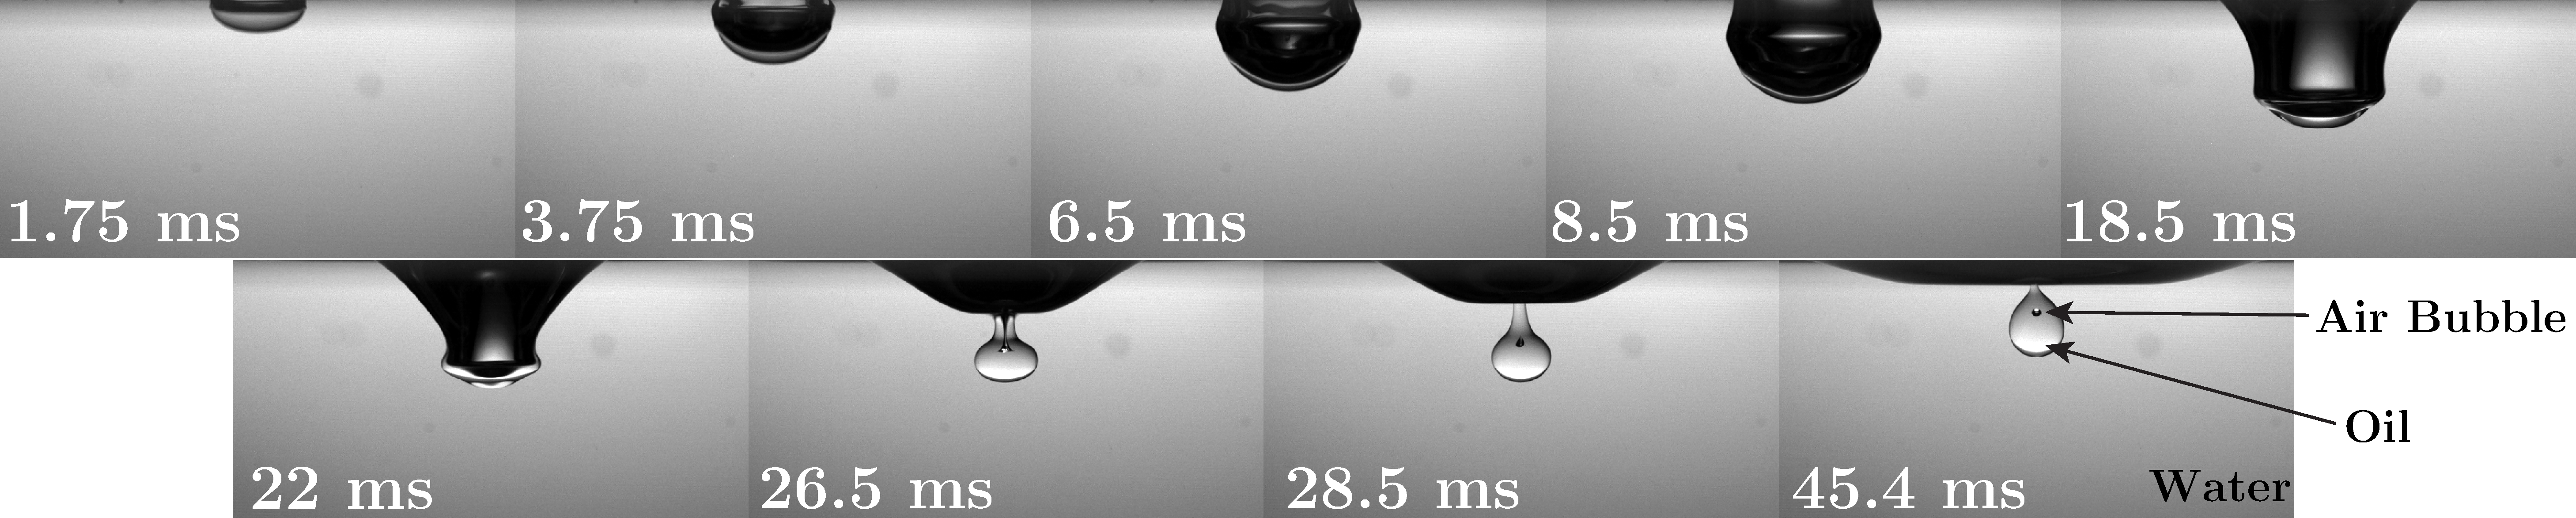
\includegraphics[width=\textwidth]{drawing.pdf}
\caption{Temporal sequence of the air-entrainment process.}
\label{Figure::Typical}
\end{center}
\end{figure}
\section*{What you will do and what you will learn?}
In the Physics of Fluids group, we are looking for enthusiastic students.
\begin{enumerate}
\itemsep0em
\item You will learn about fundamental fluid dynamics and capillary waves propagation.
\item You will get hands-on experience with Computational Fluid Dynamics (CFD).
\item You will learn how to do basic and advance data analysis.
\item You will work closely with experimentalists to understand the process.
\end{enumerate}
If you have any questions, fell free to contact \href{mailto:v.sanjay@utwente.nl}{Vatsal} or \href{mailto:u.jain@utwente.nl}{Utkarsh} (details below).
\begin{center}
\begin{tabular}{|l|l|l|}
\hline \textbf{Supervision} & \textbf{E-mail} & \textbf{Office} \\
\hline Vatsal Sanjay & \href{mailto:v.sanjay@utwente.nl}{v.sanjay@utwente.nl} & Meander 246B \\
\hline Utkarsh Jain   & \href{mailto:u.jain@utwente.nl}{u.jain@utwente.nl}& Meander 247 \\
%\hline Dr. Maziyar (Mazi) Jalaal   & \href{mailto:m.jalaal@utwente.nl}{m.jalaal@utwente.nl}&-- \\
\hline Prof. Devaraj van der Meer & \href{mailto:d.vandermeer@utwente.nl}{d.vandermeer@utwente.nl} & Meander 259  \\
\hline Prof. Detlef Lohse & \href{mailto:d.lohse@utwente.nl}{d.lohse@utwente.nl} & Meander 261  \\
\hline
\end{tabular}
\end{center}
\printbibliography
\end{document}
